\chapter{Vulkan}
Vulkan is a new generation graphics and compute API that provides high-efficiency, cross-platform access to modern GPUs used in a wide variety of devices from PCs and consoles to mobile phones and embedded platforms \cite{vulkan}. Vulkan is a much lower level API compared to OpenGL \cite{sellers:2016}; It requires the developer to deal with a lot of different hardware related aspects, from enabled GPU features to video memory management.

Vulkan also presents some very interesting features designed to solve problems of older APIs. For example, an OpenGL application has to explicitly tell the GPU what operations are executed to render the scene every frame \cite{opengl_spec}, which consumes a lot of valuable CPU time that could be used for other purposes depending on the application's nature (for example, a game could use this process time to compute artificial intelligence behavior for non-playable characters); Vulkan improves this by requiring the application to record all drawing commands in advance and possibly using multiple threads, and storing the commands in immutable objects which can, therefore, be buffered. Then, each frame, the application just needs to tell the GPU to execute the commands in those objects, saving CPU time.

\section{Debugging: validation layers}
Because graphics operations are executed on the GPU, debugging becomes a difficult task. Device drivers for older APIs included extensive error checking mechanisms in order to produce meaningful error messages to help developers. The Vulkan API, however, is designed around the idea of minimal driver overhead and one of the manifestations of that goal is that there is very limited error checking in the API by default. Even mistakes as simple as setting enumerations to incorrect values or passing null pointers to required parameters are generally not explicitly handled and will simply result in crashes or undefined behavior \cite{vulkan_tutorial}. Instead, Vulkan comes with a set of validation and debug layers as part of the Vulkan SDK and, when any subset of these layers are enabled, they insert themselves automatically into the call-chain of every Vulkan API call issued by the application to perform their job. Validation layers can also report warnings about potential incorrect or dangerous use of the API, and are even capable of reporting performance warnings that allow developers to identify places where the API is used correctly but not used in the most efficient way \cite{vulkan_validation_layers}. This allows developers to enable validity checks in debug builds to make sure that the application is built correctly, but disable them for release builds, allowing the API to run without doing any checks, improving performance.

\section{Compiling shaders}
Up until OpenGL 4.6, applications had to compile shader source code at run-time, passing a string of high-level source code to the graphics driver. While this allowed the application to run on different hardware, this also forced each GPU manufacturer to provide a GLSL compiler with the device driver. The development of the updated drivers to support new versions of the APIs would take longer, or, in some cases, support for newer versions was simply not provided \cite{apple_nopengl}.

\subsection{SPIR-V}
The "Standard Portable Intermediate Representation" version "V" (as in "Vulkan") is a binary representation of shader code which device drivers can parse more easily. Application developers, having their shaders written, must compile them into SPIR-V format before loading them in their applications. Support for SPIR-V shaders is included in OpenGL 4.6 and Vulkan 1.0 \cite{spirv_spec}.

Vulkan is not concerned about the language which was used to write the shader, as long as the provided SPIR-V code is valid. This allows shaders to be written in any shading language as long as it can be compiled into SPIR-V, which gives more flexibility to the API.

\section{Memory management}
While OpenGL drivers manage memory allocations transparently to the programmer, Vulkan not only allows but also requires that programmers allocate device memory and bind the memory to the resources used in the application. While this may increase the application's performance if the programmer takes advantage of it, it also requires the programmer to manually manage buffer alignments and aliasing. Figure \ref{fig:vulkan_mem_alloc} shows three memory allocation strategies possible with Vulkan \cite{vulkan_mem_mgmt}.

\begin{figure}[ht]
    \caption{Vulkan memory allocation strategies}
    \begin{center}
        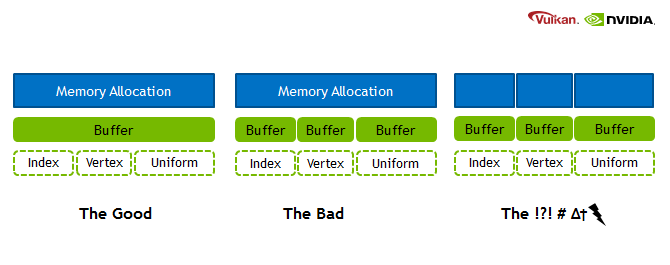
\includegraphics[width = 15cm]{figs/vulkan_memory_strategy.png}
    \end{center}
    \label{fig:vulkan_mem_alloc}
    \legend{Source: Adapted from \cite{vulkan_mem_mgmt}}
\end{figure}

The first to the left is the naive approach: for each buffer it uses a "dedicated" memory allocation. This approach is the easiest to implement, since every object allocates, binds and frees their own memory, without taking into account other objects. It is also the least optimized approach, given that it most likely will not be cache-friendly. It is also important to note that Vulkan devices have a maximum number of memory allocations that can exist simultaneously.

The approach shown in the middle ("The Bad") shows a single memory allocation with various buffers bound to it. This approach is more cache-friendly than the previous one, but it requires the programmer to deal with memory aliasing, offsets and buffer alignments.

The rightmost ("The Good") is the recommended approach. It represents a single memory allocation bound to a single buffer, with different data loaded to different areas of the buffer. This approach is the most cache-friendly and the most optimized for performance in highly-dynamic scenes, but also the most difficult to implement. This setup is possible thanks to Vulkan low-level control of offsets even inside a single buffer, allowing the developer to define "virtual buffers".

The tool developed in this work was intended to allow the user to write shaders with few objects, for the purposes of visualization only. For this reason, we opted to use the naive approach. Implementing a memory management module would not have a perceived impact on the performance of the application.

\section{Host application}
Vulkan is a low-level API and, as such, requires developers to setup a large amount of objects and configuration values before displaying anything on screen. In this section we will explain the purpose of each of these objects.

\subsection{Vulkan instance}
There is no global state in Vulkan and all per-application state is stored in a `VkInstance' object. Creating this object initializes the Vulkan library and allows the application to pass information about itself to the implementation \cite{vulkan_docs}. Applications can even define and manage multiple instances depending on their requirements.

In order to initialize a Vulkan instance object, we can first create a `VkApplicationInfo' object, which will describe our application for the driver. This structure holds the name and version of the application, and also the name and version of the engine used. This data is technically optional, but it may provide some useful information to the driver to optimize for specific applications \cite{vulkan_tutorial}. Unlike the `VkApplicationInfo', the `VkInstanceCreateInfo' structure object is not optional. It describes the instance extensions and debug layers we want to enable in our application. To make sure our application can be executed, we can check the available extensions with the function `vkEnumerateInstanceExtensionProperties' to compare against our required extensions.

During the Vulkan instance object creation we can also specify validation layers to be enabled. Available validation layers can be queried with the `vkEnumerateInstanceLayerProperties' function. The Vulkan SDK provides a standard validation layer, "VK\_LAYER\_LUNARG\_standard\_validation", which implicitly enables a range of useful diagnostic layers. In order to receive the debug messages from the validation layers, however, the application must also enable the "VK\_EXT\_debug\_report" extension, which will allow the developer to setup a callback function that will be called whenever a debug message is issued by the validation layers. To setup the debug callback function, the developer has to get a pointer to the `vkCreateDebugReportCallbackEXT', which is an extension function and therefore not included in the base API, using the `vkGetInstanceProcAddr' function.

\subsection{Physical device}
The function `vkEnumeratePhysicalDevices' returns a list of available Vulkan devices installed in the system. Basic device properties like the name, type and supported Vulkan version can be queried using `vkGetPhysicalDeviceProperties'. The support for optional features like texture compression, 64 bit floats and multi viewport rendering can be queried using `vkGetPhysicalDeviceFeatures'. Device features must be enabled before they are used by the application.

Almost every operation in Vulkan, from drawing to uploading textures, requires commands to be submitted to a queue. A queue belongs to a \emph{queue family}, and each queue family supports certain types of commands. To query queue families available in the device, there is a `vkGetPhysicalDeviceQueueFamilyProperties' function.

\subsection{Device}
The function `vkCreateDevice' takes a physical device queried and a `VkDeviceCreateInfo' object as arguments. The latter describes which physical device features we want to enable from our selected physical device and specify the queue family index and how many queues we want to create from each family. The application does not need to explicitly create the queue objects; after the device is created, the application can call the `vkGetDeviceQueue' function to get the `VkQueue' objects to which commands will be passed into for execution.

\subsection{Window surface}
In order to display images, the Vulkan API must interface with the platform specific window system. Also, since Vulkan is also a compute API, this functionality is not in its core specification, but is part of the "VK\_KHR\_surface" extension. Window systems also vary for each platform so, in order to create the proper surface object, we also need to enable the platform-specific surface extension ("VK\_KHR\_win32\_surface" for Windows, for example).

\subsection{Swap chain}
Unlike OpenGL, Vulkan does not have the concept of a "default framebuffer", hence it requires a structure to own the buffers where images will be rendered before they are displayed on screen. This structure is the swap chain, and it must be explicitly created. This requires the "VK\_KHR\_swapchain" device extension enabled. The swap chain is essentially a queue of images that are waiting to be presented on the screen.

Each physical device presents different capabilities in its swap chain. These include the maximum number of images the swap chain can hold, the pixel formats supported and presentation modes. The presentation modes are \cite{vulkan_tutorial}:
\begin{itemize}
    \item \texttt{VK\_PRESENT\_MODE\_IMMEDIATE\_KHR}: Images submitted by your application are transferred to the screen right away. May result in tearing;
    \item \texttt{VK\_PRESENT\_MODE\_FIFO\_KHR}: The swap chain is a queue where the display takes an image from the front of the queue when the display is refreshed and the program inserts rendered images at the back of the queue. If the queue is full then the program has to wait. This is most similar to vertical sync as found in modern games. This is the only mode that is guaranteed to be supported;
    \item \texttt{VK\_PRESENT\_MODE\_FIFO\_RELAXED\_KHR}: This mode only differs from the previous one if the application is late and the queue was empty at the last vertical blank. Instead of waiting for the next vertical blank, the image is transferred right away when it finally arrives. This may result in visible tearing;
    \item \texttt{VK\_PRESENT\_MODE\_MAILBOX\_KHR}: This is another variation of the second mode. Instead of blocking the application when the queue is full, the images that are already queued are simply replaced with the newer ones. This mode can be used to implement triple buffering, which avoids tearing with significantly less latency issues than standard vertical sync that uses double buffering.
\end{itemize}

\subsection{Depth resources}
In Vulkan, the depth buffer is an image object which the developer has to create explicitly using special formats that are defined for depth images. Device memory must be allocated for the image and bound to it, and an image view also needs to be created to describe how the image will be used. After creation, the image must also be transitioned to a layout optimal for depth attachment before it can be used as depth buffer.

\subsection{Render pass}
A render pass represents a collection of attachments, subpasses, and dependencies between the subpasses, and describes how the attachments are used over the course of the subpasses \cite{vulkan_docs}.

\subsection{Framebuffer}
The attachments specified in the render pass creation are bound into a framebuffer object. This object references all the image view objects that represent the attachments in the render pass. Since the swap chain has many different images (and image views), applications must also create a framebuffer for each image view of the swap chain.

\subsection{Command buffers and command pools}
As we mentioned, operations like drawing and memory transfers are not executed with function calls in Vulkan. Instead, the commands are recorded in command buffers, which are then submitted to a queue for execution.

Command buffers are not created directly, but they are allocated from command pools which will manage the memory used by the command buffers. Each command pool can only execute commands on a single queue family; command buffers allocated from a pool cannot simply execute any command, because the commands will be executed by a queue family which may not support the operations.

\subsection{Buffers}
Data is passed from the host application to the graphics pipeline via buffer objects. Buffers must have device memory allocated and bound to them in order to work, and will be used to pass vertex attributes, vertex index data when available, and uniform values. Uniform buffers are generally updated every frame.

\subsection{Images, image views and samplers}
Much like buffers, in order to be accessed by shaders, images must be created and device memory must be allocated and bound to them. There is also the need to create an image view, an object that describes how to access the image and which part of the image to access. Sampler objects will determine how the shaders will sample the pixels of the image, determining filtering and address mode, for example. In Vulkan, images and samplers are distinct objects, which allows the same image to be accessed in shader code with different samplers, using different configuration values. This feature can be used to reduce memory usage.

\subsection{Descriptor set layout, descriptor pool and descriptor set}
The descriptor set layout describes the bindings that are used in the shaders, whether they bind a uniform buffer object or an image sampler, and at which stages each binding is available.

The descriptor pool holds a pool of descriptor sets to be allocated; it requires the number of uniform buffers and image samplers, but is not concerned about the size of these structures.

The descriptor set layout is just a description of what types of descriptors can be bound, but no uniform buffers are referenced. The descriptor set specifies a buffer to be bound in the uniform buffer descriptor.

\subsection{Pipeline}
In order to create the `VkPipeline' object, one first needs to create a `VkPipelineLayout' object. The pipeline layout defines the interface of the pipeline object with our application, that is, it holds a reference to the descriptor set layout object. Developers also create objects that will configure every stage in the graphics pipeline:

\begin{itemize}
    \item \texttt{VkPipelineVertexInputStateCreateInfo}
    \item \texttt{VkPipelineInputAssemblyStateCreateInfo}
    \item \texttt{VkPipelineViewportStateCreateInfo}
    \item \texttt{VkPipelineRasterizationStateCreateInfo}
    \item \texttt{VkPipelineMultisampleStateCreateInfo}
    \item \texttt{VkPipelineDepthStencilStateCreateInfo}
    \item \texttt{VkPipelineShaderStageCreateInfo}
    \item \texttt{VkPipelineColorBlendStateCreateInfo}
\end{itemize}

Each of the structures mentioned above have a set of possible configurations which will determine, for example, the topology used when interpreting the vertex data (points, lines, triangles), which polygon mode to use in rasterization (points, lines, fill), line width, back face culling, depth comparison operation and alpha blending.
